\chapter{Deep learning}\label{ch-17}

This lecture introduces \textbf{deep learning} (DL) from the point of
view of the course: not the details of the architectures for
applications (which will be seen in the subsequent courses of the AI
curriculum, such as Pattern Recognition and NLP), but an
\textbf{overview} of networks with many layers, the concepts that make
them effective (\textbf{are many layers really needed?},
\textbf{representation learning}, \textbf{distributed representations})
and the main training \textbf{techniques}, many of which are also
useful in the ``basic'' case.

\section{What is deep learning}\label{che-cosuxe8-il-deep-learning}

\begin{boxnote}{LeCun, Bengio, Hinton, \emph{Nature} (2015)}

\emph{``Deep learning allows computational models that are composed of
multiple processing layers to learn representations of data with
multiple levels of abstraction. These methods have dramatically
improved the state-of-the-art in speech recognition, visual object
recognition, object detection and many other domains.''}

\end{boxnote}

\subsection{A bit of history}\label{un-po-di-storia}

Since about 2010 deep learning has had a strong impact on industry, due
to three factors:

\begin{itemize}
\tightlist
\item
  \textbf{large datasets} available (millions of images);
\item
  \textbf{computing power} (GPUs are the enabling factor);
\item
  \textbf{new ideas} to make training easier.
\end{itemize}

Learning with deep architectures is no longer ``infeasible''. The new
state-of-the-art results in speech recognition, machine translation
(Google Neural Translator since 2016, DeepL) and image recognition have
attracted a great many researchers. In the past an improvement was
expected by changing the scale of models and data, but not necessarily
such a leap in performance. All the big IT companies today base their
research and development strategies on these approaches.

\subsection{The general framework}\label{il-quadro-generale}

DL is a \textbf{general framework} that includes different models:

\begin{itemize}
\tightlist
\item
  \textbf{deep neural networks} (MLPs with many layers);
\item
  \textbf{convolutional networks} (winners in computer vision);
\item
  \emph{deep belief networks} and generative approaches;
\item
  \textbf{recurrent} and \textbf{recursive} networks;
\item
  \ldots{}
\end{itemize}

It is contrasted with \textbf{``shallow'' models}, for example networks
with fewer than 3 layers. The aspects common to the various approaches
are:

\begin{itemize}
\tightlist
\item
  \textbf{several layers} of \textbf{non-linear} processing units;
\item
  learning (supervised or unsupervised) of \textbf{feature
  representations} in each layer, with the layers forming a
  \textbf{hierarchy} from low-level to high-level features (different
  levels of abstraction);
\item
  hence, a \textbf{hierarchical, sparse and distributed representation}
  of the data.
\end{itemize}

(The differences depend on the specific models: max pooling in CNNs,
energy-based training in RBMs, etc.)

\subsection{The conceptual ingredients: hierarchical
abstraction}\label{gli-ingredienti-concettuali-astrazione-gerarchica}

Recall XOR solved with two layers
(\href{06\%20-\%20Reti\%20neurali\%20(parte\%201)\%20-\%20dal\%20neurone\%20al\%20MLP}{06
- Neural networks (part 1) - from the neuron to the MLP}): the hidden
layer creates an \textbf{internal re-representation} that makes the
task easy for the output layer, and this composition of intermediate
operations can be extended over many levels of abstraction.

\begin{itemize}
\tightlist
\item
  Unsupervised or semi-supervised \textbf{feature learning} and
  hierarchical feature extraction, \textbf{instead of feature
  engineering} (features extracted by hand, from experience, such as
  texture in images): we move to the concept of \textbf{learning
  representations of the data}.
\item
  \textbf{Increasing levels of abstraction} through the layers. An
  image can be represented as a vector of pixel intensities, or more
  abstractly as a set of edges, regions of particular shape, etc.:
  \textbf{edges form motifs, motifs assemble into parts, parts form
  objects}\ldots{} over many levels.
\item
  It works best when the input has some form of \textbf{structure}
  (spatial, temporal, \ldots).
\end{itemize}

\begin{figure}[htbp]
\centering
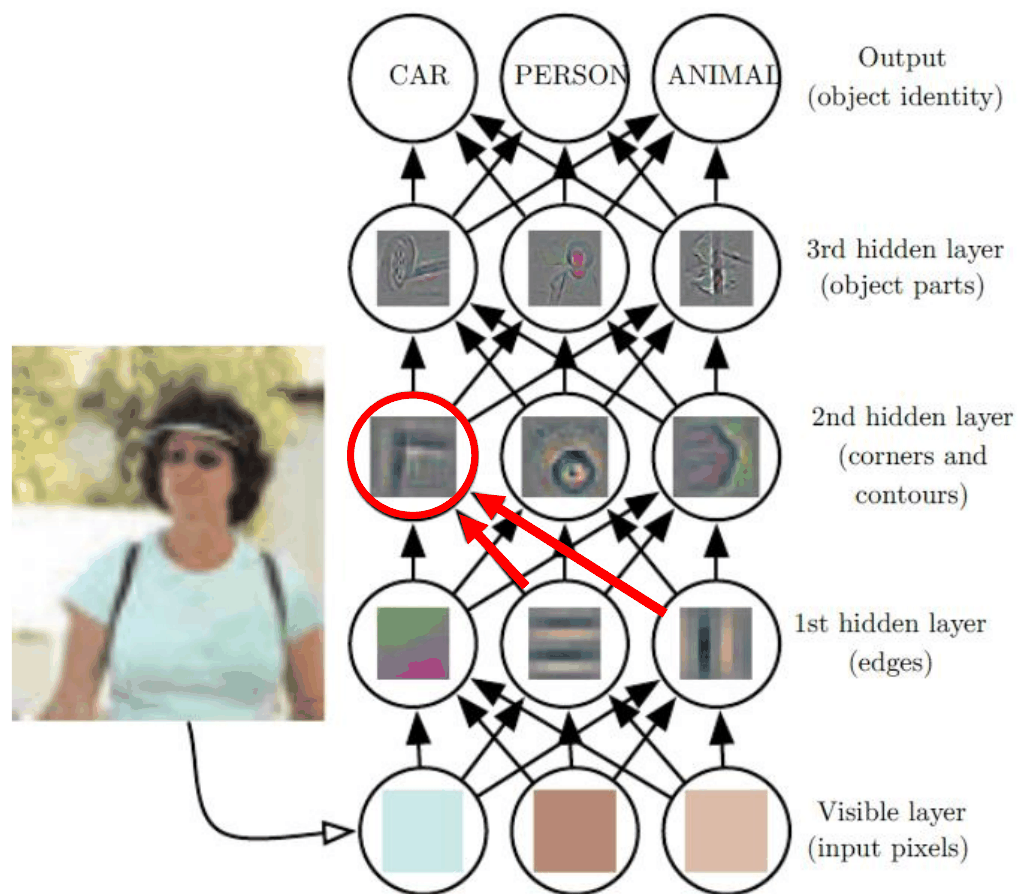
\includegraphics[width=0.63\linewidth,height=0.42\textheight,keepaspectratio]{images/17-deep_gerarchia.png}
\caption{From pixels to the identity of the object: a series of hidden
layers extracts increasingly abstract features (edges → corners and
contours → object parts).}
\end{figure}

Deep learning solves the difficulty of a complicated mapping (pixels →
identity) \textbf{by breaking it into a series of simple nested
mappings}, each described by a different layer. The new representation
\textbf{simplifies classification} in the last layer. There are
analogies with the biological visual system.

In networks these abstract features \textbf{are learned from
examples}: with backpropagation, the error on the output layer (for
example to distinguish cars and people) propagates through the deltas
across the layers, and the units specialise to provide high-level
features useful for that purpose (the wheel for the car, the hand for
the person\ldots). The link between the automatically developed
features and reality is a fascinating aspect; and surprisingly the
first filters extract horizontal or vertical lines, just as a simple
linear convolutional filter would.

\begin{figure}[htbp]
\centering
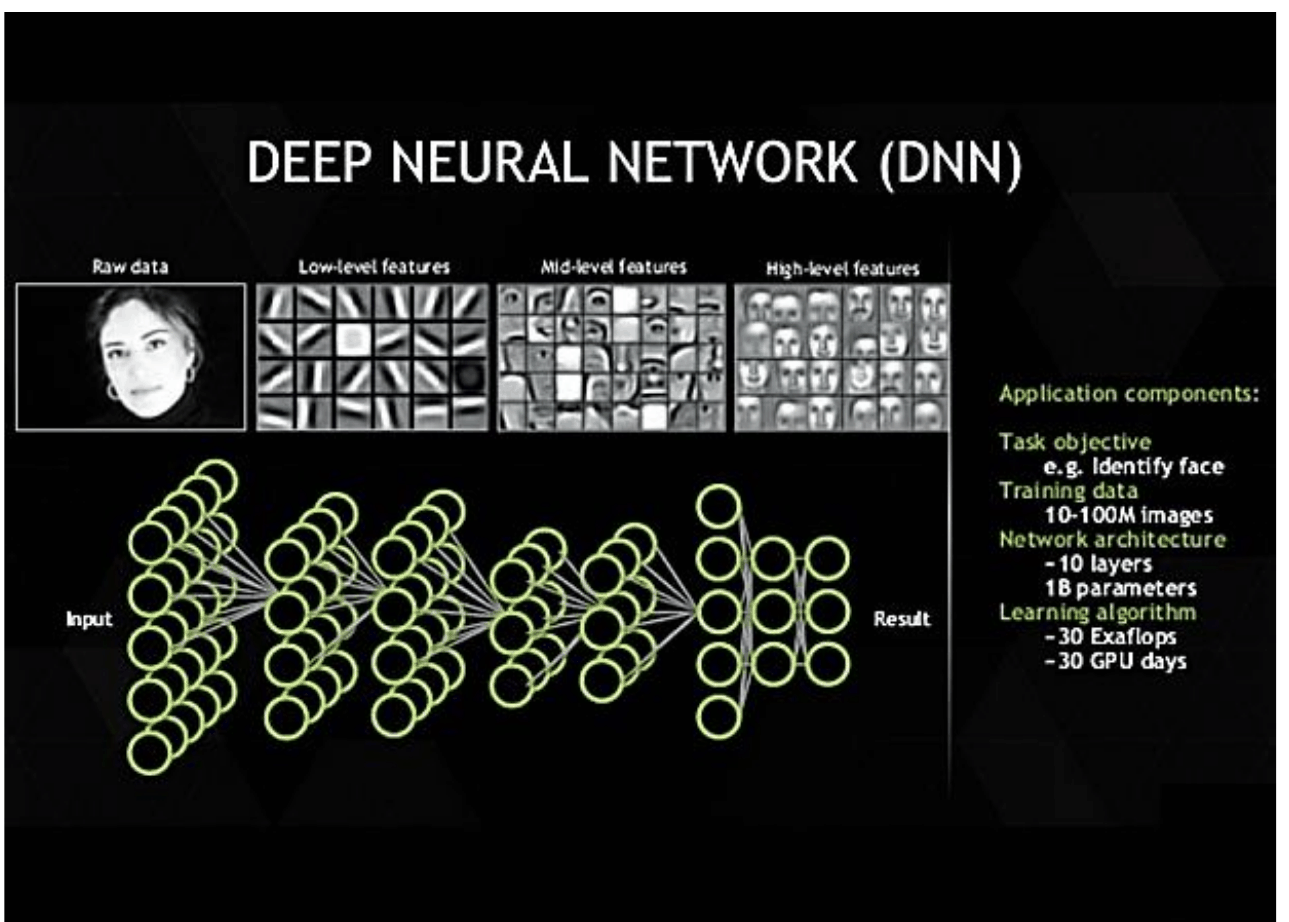
\includegraphics[width=0.69\linewidth,height=0.42\textheight,keepaspectratio]{images/17-deep_dnn.png}
\caption{Another example: low-, mid- and high-level features in a deep
network for faces.}
\end{figure}

\subsection{Combining to
generalise}\label{combinare-per-generalizzare}

Abstract features can be \textbf{reused} at higher levels (e.g.\
gender, glasses\ldots) and \textbf{combined} to generalise to cases
never seen in training: if the network has seen women without glasses
and men with glasses, it can easily represent a woman with glasses as
well.

\begin{figure}[htbp]
\centering
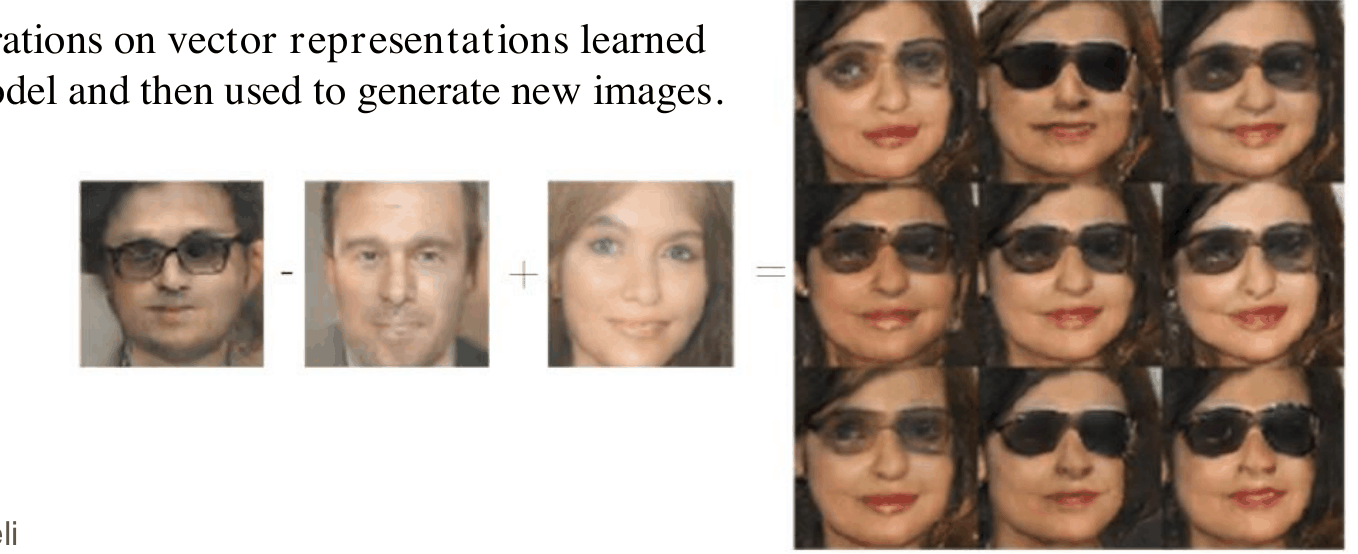
\includegraphics[width=0.74\linewidth,height=0.42\textheight,keepaspectratio]{images/17-deep_occhiali.png}
\caption{Operations on the vector representations learned by the model
and used to generate new images: ``man with glasses − man + woman =
woman with glasses''.}
\end{figure}

The same happens in language: in the vector space developed by the
inner layers of a deep model,

\begin{itemize}
\tightlist
\item
  \(\text{Rep}(\text{king}) - \text{Rep}(\text{male}) + \text{Rep}(\text{female}) \approx \text{Rep}(\text{queen})\):
  the difference between ``king'' and ``male'' captures the concept of
  monarchy;
\item
  \(\text{Rep}(\text{Paris}) - \text{Rep}(\text{France}) + \text{Rep}(\text{Poland}) \approx \text{Rep}(\text{Warsaw})\):
  the difference captures the concept of capital.
\end{itemize}

\section{Are many layers really
needed?}\label{servono-davvero-molti-strati}

\subsection{An example from logic
circuits}\label{un-esempio-dai-circuiti-logici}

The general idea (\textbf{no-flattening}): \emph{when a function is
represented compactly by a deep architecture, it might require a very
large architecture to be represented by an insufficiently deep one.}

A \textbf{two-layer} logic circuit can represent \textbf{any} Boolean
function, written as a sum of products (disjunctive normal form): AND
gates in the first layer (with possible negation of the inputs) and an
OR gate in the second. But \textbf{with depth-two circuits, most
Boolean functions require an exponential number of gates} (with respect
to the input size).

\begin{boxexample}{The parity function}

\textbf{Odd parity} extends XOR to \(N\) inputs: it returns 1 if and
only if the number of 1s among the \(N\) bits is odd. (NOTs are also
assumed to be available; with 2 inputs 3 gates are enough.)

\textbf{With 2 layers} all the positive configurations must be listed:
for 3 inputs,
\(x_1x_2x_3 + x_1\bar x_2\bar x_3 + \bar x_1x_2\bar x_3 + \bar x_1\bar x_2x_3\)
(1 if the input is 111, 100, 010 or 001), i.e.\ 4 AND + 1 OR = 5 gates.
For 4 inputs 9 gates are needed, for 8 inputs \textbf{129 gates}, for
\(N\) inputs \(2^N/2 + 1 = 2^{N-1} + 1\) gates: an
\textbf{exponential} number.

\textbf{With \(\log N\) layers} a \textbf{complete binary tree} of XORs
is used: a tree with \(N\) leaves has \(N - 1\) internal nodes, each an
XOR of 3 AND/OR gates, for a total of \(3(N-1)\) gates, a
\textbf{polynomial} number. For 8 inputs \(3 \times 7 = 21\) gates are
enough against the 129 of the 2-layer solution.

\end{boxexample}

\begin{figure}[htbp]
\centering
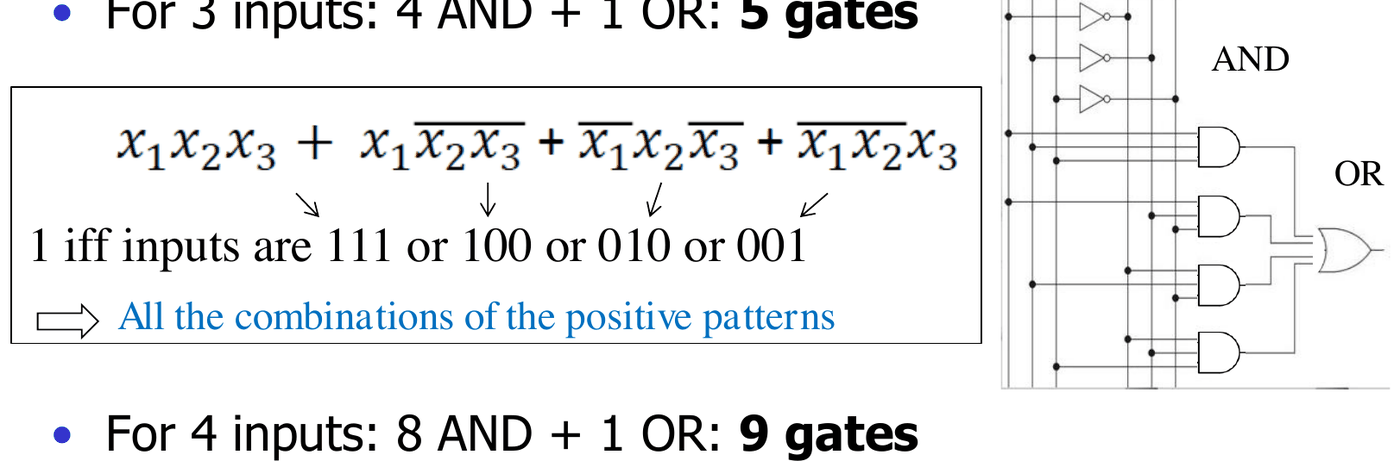
\includegraphics[width=0.80\linewidth,height=0.42\textheight,keepaspectratio]{images/17-deep_parita-2strati.png}
\caption{Parity with 2 layers: an exponential number of gates.}
\end{figure}

\begin{figure}[htbp]
\centering
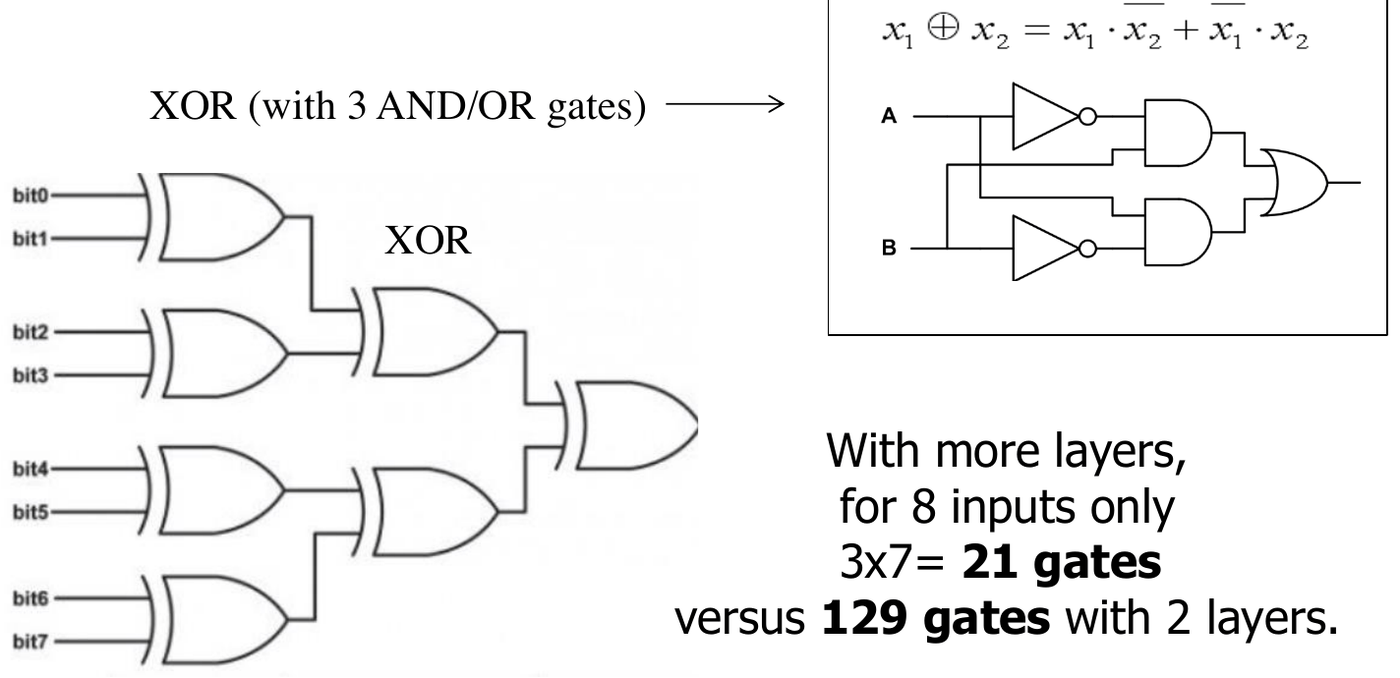
\includegraphics[width=0.74\linewidth,height=0.42\textheight,keepaspectratio]{images/17-deep_parita-albero.png}
\caption{Parity with \(\log N\) layers: a tree of XORs with a polynomial
number of gates.}
\end{figure}

This, however, \textbf{does not hold for all classes of functions}:
characterising the classes that gain an (exponential) advantage from a
multi-layer structure is an open research problem.

\subsection{The case of neural
networks}\label{il-caso-delle-reti-neurali}

Recall that the \textbf{universal approximation theorem} shows that one
hidden layer is enough in general, but it does not guarantee that a
\textbf{small} number of units is enough. There are, however,
\textbf{no-flattening} results (on efficiency, not on expressiveness):

\begin{enumerate}
\def\labelenumi{\arabic{enumi}.}
\tightlist
\item
  \textbf{shallow networks}: there are cases in which the
  implementation with a single hidden layer requires an
  \textbf{exponential} number of units (with respect to the input
  dimension \(n\)) or of non-zero weights. It is easy to see in the
  binary case: Boolean functions on \(\{0,1\}^n\) are \(2^{2^n}\), and
  in the worst case one hidden unit may be needed for each input
  configuration to be distinguished (as in the parity example). It is
  not only a problem of network size: it also means that it becomes
  \textbf{hard to learn with few examples} (and this is the most
  relevant point for ML);
\item
  \textbf{no-flattening of deep networks}: there are families of
  functions that can be approximated efficiently with depth greater
  than \(d\), but that require a much larger model (up to an
  exponential gain) if the depth is at most \(d\). Examples for logic
  gates (1986), networks with standard activations (1990--1994), ReLU
  (2014)\ldots{}
\end{enumerate}

The question remains: is it easy to train an MLP with many layers? (See
the techniques later.)

\begin{boxnote}{Theoretical analysis (open research)}

\textbf{No-flattening theorems} identify compositional functions that a
deep network implements well and that cannot be implemented with the
same efficiency by ``flattening'' the network (for example going from a
linear to an exponential number of units). But there is no guarantee
that a given task has this property: a complete list of no-flattening
theorems would say exactly when deep networks are more efficient than
shallow ones.

\end{boxnote}

\subsection{Why: compositionality}\label{perchuxe9-la-composizionalituxe0}

Deep networks can exploit the \textbf{compositionality of internal
representations}: there is an exponential gain in representational
power because the simple concepts represented in one layer are used as
\textbf{primitives} by the next layer to represent more complex
concepts, avoiding the explicit and combinatorial representation (and
learning) of the features.

For example, one must learn the individual words or sub-patterns, but
not directly all their possible combinations: one can learn without
seeing all the configurations. And perhaps nature itself (not only
images and language) has a hierarchical structure (phenomena observed
at different scales in space and time).

\begin{boxtip}{Less is more!}

Deep networks should not be seen as \textbf{huge} models compared to
small shallow models (just because in applications one sees gigantic
instances: deep does not mean large). They can be seen as
\textbf{compact} models compared to potentially much larger shallow
models for the same task (even exponentially). So they are ``something
less'' and more efficient. And not only for computational reasons:
\textbf{fewer units and fewer weights help learning} on complex tasks,
making it possible to generalise well with \textbf{fewer examples}
(i.e.\ making it feasible). A ``small deep network'' of 50,000 units
can replace a ``huge shallow network'' of one million units.

\end{boxtip}

\subsection{The inductive bias}\label{il-bias-induttivo}

Choosing a deep model encodes a \textbf{very general belief}: that the
function to be learned is a \textbf{composition of simpler functions}
(or of nested factors of variation). If the task matches this bias, the
deep form is suitable, and generalisation turns out better precisely
thanks to the many layers.

Typically hierarchical tasks: the structure of \textbf{images}
(composition of graphical parts), the structure of \textbf{language}
(text and speech), perhaps music; new fields are being discovered. But
not necessarily all data and tasks! It is in any case a much more
\textbf{general} bias than ad hoc constraints for specific tasks (such
as hand-chosen \(\phi\) in LBE or engineered features). But, again,
nothing is magic without assumptions.

\begin{figure}[htbp]
\centering
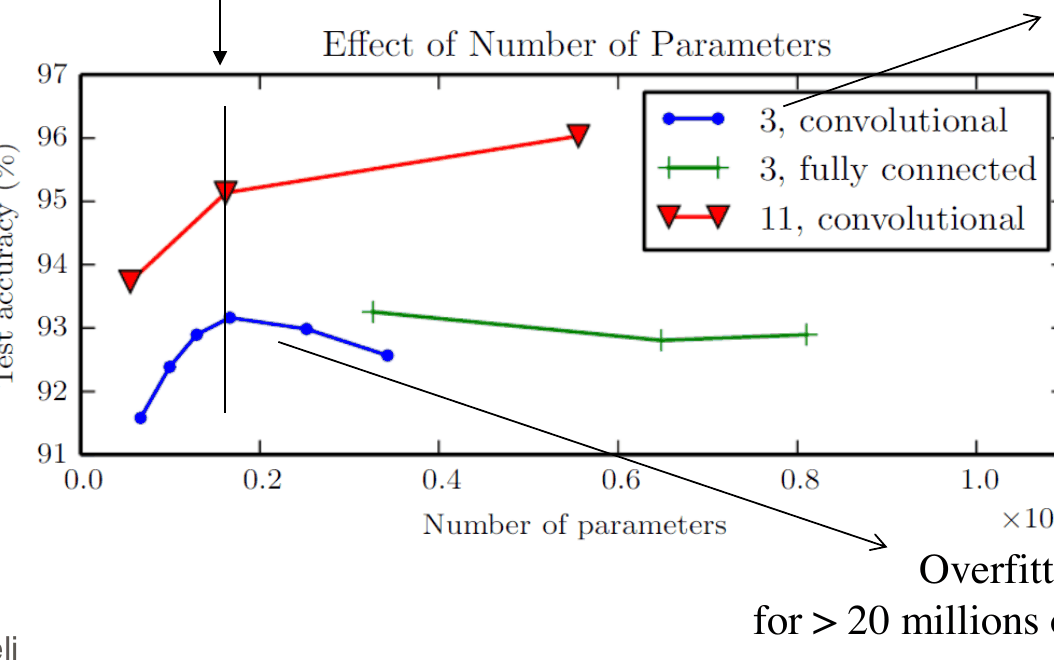
\includegraphics[width=0.57\linewidth,height=0.42\textheight,keepaspectratio]{images/17-deep_svhn.png}
\caption{Empirical results (SVHN, ICLR 2014): with the same number of
parameters, deeper networks generalise better.}
\end{figure}

When the task matches the bias, deeper models tend to work better:
generalisation is better than a model with fewer layers and \textbf{the
same number of units/weights}.

\subsection{Curse of dimensionality and
bias}\label{maledizione-della-dimensionalituxe0-e-bias}

Other arguments in favour of deep models concern the \textbf{curse of
dimensionality} and \emph{manifold learning} (the distribution of real
images and texts seems concentrated on a manifold that occupies only a
small fraction of the volume of all possible random images or texts).

\begin{itemize}
\tightlist
\item
  Many learners rely on \textbf{local approximations} (a local
  \emph{smoothness} prior): K-NN, local kernels, decision
  trees\ldots{} But often this is not enough: examples are needed to
  generalise in the neighbourhood of each region, and in high dimension
  a huge number of examples is needed to cover the whole space. To
  distinguish \(O(k)\) regions, all these methods require \(O(k)\)
  examples.
\item
  To work with \(O(k)\) examples on an \textbf{exponential} (in \(k\))
  number of regions, i.e.\ to generalise \textbf{non-locally},
  additional assumptions on the data-generating distribution (an
  inductive bias) are needed.
\item
  One could make strong, specific assumptions for each task (losing
  generality). Deep learning instead chooses a \textbf{general} bias,
  related to the \textbf{composition of functions}: the data are
  assumed to be generated by the composition of factors or features,
  potentially over several levels of a hierarchy. When the assumption
  is true, one obtains a potentially exponential gain between the
  number of examples and the number of distinguishable regions, one
  generalises non-locally, and one learns with fewer examples.
\end{itemize}

\subsection{Practical issues}\label{questioni-pratiche}

How many layers? How many units? There is still no general answer (it
is a model selection problem). In general deep networks often use fewer
units per layer, hence fewer parameters and less data to generalise
well; but many layers can be \textbf{harder to optimise}. The
hyperparameters of these very large models may be too many:
\textbf{experience} makes the difference in fixing many architectural
aspects.

\section{Representation learning}\label{representation-learning}

\begin{boxdefinition}{Representation learning}

\emph{``Representation learning is a set of methods that allows a
machine to be fed with raw data and to automatically discover the
representations needed for detection or classification.''} (LeCun,
Bengio, Hinton, 2015)

\end{boxdefinition}

Deep learning methods are representation learning methods with
\textbf{multiple levels} of representation (representations expressed
in terms of other, simpler ones). But the concept is more abstract and
applies to many models (for example neural networks in general). Note
that we speak of learning the representation mainly for \textbf{raw
data} (images, text strings), not when a small set of features is
already provided.

\subsection{Basic ideas}\label{idee-di-base}

\begin{itemize}
\tightlist
\item
  Many information processing tasks are easy or very hard
  \textbf{depending on how the information is represented} (this holds
  across computer science).
\item
  In ML, \textbf{a good representation is one that makes the subsequent
  learning task easier}.
\item
  Designing features by hand is hard: whole decades of work for some
  communities (language, images). It is equivalent to hand-engineering
  the \(\phi(\mathbf{x})\) of LBE.
\item
  Supervised learning of an MLP leads to an \textbf{automatic
  representation} in each hidden layer, with properties that make the
  task of the output layer easier (XOR!). That is,
  \(\phi(\mathbf{x}, \mathbf{w})\) is learned by finding the best
  \(\mathbf{w}\).
\item
  In CNNs the raw image is used as input and the model learns to
  extract the features salient for the task, without patterns or
  features specified in advance.
\end{itemize}

How to obtain or exploit the hidden representations (besides the full
training of MLPs and CNNs)?

\begin{itemize}
\tightlist
\item
  \textbf{Obtaining them} (historical case): with
  \textbf{semi-supervised} learning a representation is learned from
  unlabelled data and used for supervised tasks →
  \textbf{pre-training}.
\item
  \textbf{Exploiting them}: the learned representation is used for
  other tasks → \textbf{transfer learning}.
\end{itemize}

\subsection{Pre-training}\label{pre-training}

\emph{Greedy layer-wise unsupervised pretraining} (around 2006) was the
first approach that made it possible to train deep supervised networks
(apart from CNNs and RNNs). \textbf{Unsupervised} learning is used to
capture the shape of the input distribution, \textbf{layer by layer},
and the network is initialised this way, making overall training easier
(instead of immediately doing \emph{end-to-end} training with gradient
descent, which was difficult for deep models).

Why does it help? Each layer is optimised independently in an
unsupervised way, constituting a pre-training for the final
\textbf{fine-tuning}. It works both as a \textbf{good initialisation
strategy} and as \textbf{regularisation}: not in the sense of a simpler
model, but of discovering features that capture the regularities of the
data. If the true functions are complicated and shaped by the
regularities of the input distribution, unsupervised learning can be a
more appropriate regulariser. It also reduces the \textbf{variance} of
the estimation process (pre-trained models tend to end up in a smaller
region).

\subsubsection{Autoencoder}\label{autoencoder}

\begin{boxdefinition}{Autoencoder}

An \textbf{autoencoder} is a neural network trained to \textbf{copy its
input to its output}. Internally it has a hidden layer \(\mathbf{h}\)
that describes a \textbf{code} to represent the input. It consists of
an \textbf{encoder} \(\mathbf{h} = f(\mathbf{x})\) and a
\textbf{decoder} that produces the reconstruction
\(\mathbf{r} = g(\mathbf{h})\).

\end{boxdefinition}

\begin{figure}[htbp]
\centering
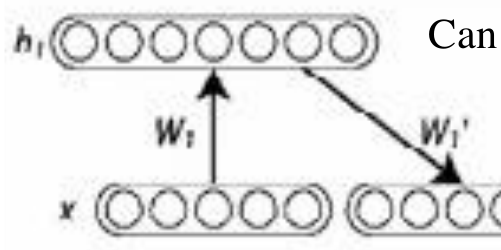
\includegraphics[width=0.34\linewidth,height=0.42\textheight,keepaspectratio]{images/17-deep_autoencoder.png}
\caption{An autoencoder: encoder (W₁) and decoder (W₁').}
\end{figure}

\begin{itemize}
\tightlist
\item
  \textbf{Undercomplete}: the hidden layer is \textbf{smaller} than the
  input, and the architectural constraint forces the network to capture
  the most salient features. (With a linear decoder and squared loss
  one obtains PCA.)
\item
  \textbf{Overcomplete}: the hidden layer is \textbf{larger} than the
  input, but a regularisation is used that imposes sparsity, robustness
  to noise or other properties, beyond the trivial ability to copy.
\item
  It is \textbf{unsupervised} learning.
\end{itemize}

Example of use: \textbf{denoising autoencoders} and auto-associative
memories. It is trained on images looking for a good representation
(``\emph{a good representation is one that can be obtained robustly
from a corrupted input and that will be useful for recovering the clean
input}''), then the original image is recovered by presenting a noisy
version of it and repeating the encoding and decoding phases.

\subsubsection{The pre-training algorithm
(Bengio)}\label{lalgoritmo-di-pre-training-bengio}

\begin{boxabstract}{Layer-wise pre-training}

\begin{enumerate}
\def\labelenumi{\arabic{enumi}.}
\tightlist
\item
  Train the first layer as an \textbf{auto-associator} to minimise the
  reconstruction error of the raw input (unsupervised: unlabelled
  examples are enough).
\item
  Use the outputs of the hidden units as input for another layer, also
  trained as an auto-associator.
\item
  Repeat until the desired number of layers.
\item
  Use the output of the last hidden layer as input for a supervised
  layer, initialised (randomly or with supervised training, keeping the
  rest fixed).
\item
  \textbf{Fine-tune} all the parameters with respect to the supervised
  criterion.
\end{enumerate}

The hope is that the unsupervised initialisation has brought the
parameters into a region from which local descent reaches a good local
optimum.

\end{boxabstract}

Autoencoders are used as RBMs (\emph{Restricted Boltzmann Machines},
energy-based models, in Hinton's \emph{deep belief networks}) or as
stacked (denoising) autoencoders (Bengio, 2007).

\begin{boxnote}{Is pre-training still needed?}

Pre-training made it possible to \textbf{kick-start} deep learning and
still gives improvements in some tasks (especially NLP, where it allows
exploiting large text corpora to learn distributed word
representations). But it is hard to manage (hyperparameters split into
two phases) and today \emph{``unsupervised pre-training is largely
abandoned''} (DL book, ch.\ 15): modern techniques are enough for good
\textbf{end-to-end} training from scratch with backpropagation.

\end{boxnote}

\begin{boxnote}{Encoders and decoders today}

\begin{itemize}
\tightlist
\item
  \textbf{Variational autoencoders} use a Bayesian framework: the
  latent space is a mixture of distributions instead of a fixed
  vector.
\item
  \textbf{Neural machine translation} is implemented with
  encoder-decoder architectures in which the output does not coincide
  with the input but is in another language.
\item
  \textbf{Transformers} (such as GPT, \emph{Generative Pre-trained
  Transformer}) are encoder/decoder networks with an
  \textbf{attention} mechanism. One can use only the encoder (BERT, for
  various NLP tasks) or only the decoder, for generative purposes (the
  GPT series for autoregressive text generation).
\end{itemize}

\end{boxnote}

\subsection{Transfer learning}\label{transfer-learning}

The representation discovered by a model is used to \textbf{improve
another model}, assuming that there are useful features in different
contexts or tasks, corresponding to common underlying factors.
Different forms (they are real sub-fields of ML, not just
terminology):

\begin{itemize}
\tightlist
\item
  from autoencoder to classifier (as above);
\item
  \textbf{multi-task learning}: same inputs, different targets (an
  implicit regularisation);
\item
  \textbf{domain adaptation}: different input domain but shared
  features (e.g.\ sentiment analysis on video and smartphone reviews);
\item
  reuse of \textbf{pre-trained models} on larger datasets.
\end{itemize}

\begin{boxexample}{Transfer learning with AlexNet}

AlexNet is a CNN trained on about 1.2 million ImageNet images in 1000
categories: it has learned \textbf{rich representations} for a wide
range of images, with low-level primitives shared across different
images. It has 5 convolutional layers and 3 fully connected ones. For a
new task one \textbf{replaces the last 3 layers} and trains only those
with a few new images, or does \textbf{fine-tuning} of the whole
network. Many pre-trained CNNs (VGG, ResNet, GoogLeNet\ldots) are
available in the libraries.

\end{boxexample}

\section{Distributed
representations}\label{rappresentazioni-distribuite}

\begin{boxdefinition}{Distributed representation}

\emph{``In a distributed representation the elements (the features)
are not mutually exclusive and their many configurations correspond to
the variations seen in the observed data.''} (LeCun, Bengio, Hinton,
2015)

\end{boxdefinition}

Deep learning methods exploit distributed representations over several
levels, but the concept applies to many models (neural networks in
general, on the hidden units; probabilistic graphical models, with
several latent variables).

\begin{figure}[htbp]
\centering
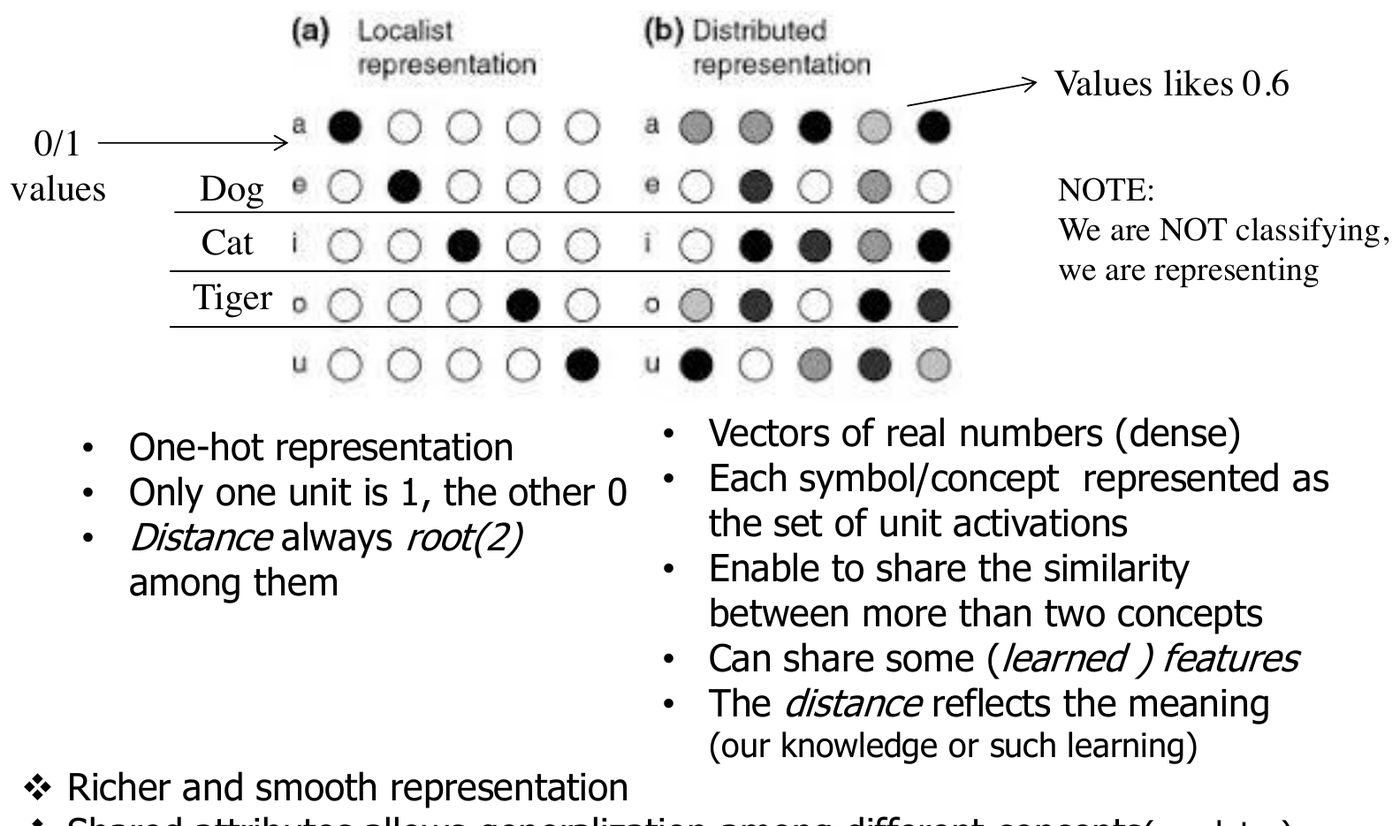
\includegraphics[width=0.74\linewidth,height=0.42\textheight,keepaspectratio]{images/17-deep_distribuita.png}
\caption{Symbolic (one-hot) and distributed representation.}
\end{figure}

{\def\LTcaptype{none} % do not increment counter
\begin{longtable}[]{@{}
  >{\raggedright\arraybackslash}p{(\linewidth - 2\tabcolsep) * \real{0.5000}}
  >{\raggedright\arraybackslash}p{(\linewidth - 2\tabcolsep) * \real{0.5000}}@{}}
\toprule\noalign{}
\begin{minipage}[b]{\linewidth}\raggedright
Symbolic (one-hot)
\end{minipage} & \begin{minipage}[b]{\linewidth}\raggedright
Distributed
\end{minipage} \\
\midrule\noalign{}
\endhead
\bottomrule\noalign{}
\endlastfoot
only one unit is 1, the others 0 & (dense) vectors of real numbers \\
distance always \(\sqrt{2}\) between different concepts & each concept
is the set of activations of all the units \\
& similarity can be shared among more than two concepts \\
& (learned) features can be shared \\
& distance reflects meaning \\
\end{longtable}
}

Beware: here we are \textbf{not classifying}, we are
\textbf{representing}. Distributed representations are richer and
smoother, and shared attributes make it possible to generalise across
different concepts.

\textbf{Input or internal representation?} The discussion is general,
but learning acts on the \textbf{internal} representation. A
distributed representation at the \textbf{input} is used only if domain
knowledge allows it to be fixed (rare and difficult; fixing it
arbitrarily can harm the task). In general a (non-informed) one-hot
input is used anyway and the model is left to develop
\textbf{internally} the necessary distributed representation.

\subsection{Counting the difference}\label{contare-la-differenza}

Four concepts: blue car, blue bike, red car, red bike. 4 neurons are
not needed: \textbf{2} are enough (\(2^2\) concepts), one for
blue/red and one for car/bike. And the neuron describing ``red'' learns
red from images of both cars and bikes, not just from a specific
category.

In general, with \(n\) features of \(k\) values a distributed
representation describes \(k^n\) different concepts (for example
\(2^n\) binary configurations), versus the \(n\) of a symbolic one-hot
representation. A unique code can be assigned to an
\textbf{exponential} number of regions: models with distributed
representations (such as networks with hidden units) distinguish
exponentially more regions than non-distributed ones.

Models based on \textbf{non-distributed} representations: K-NN (one or
a few prototypes per input, without sharing information with the whole
training set), RBF kernels (they reduce to K-NN, as seen for SVMs),
Gaussian mixtures, decision trees (only one leaf is activated).

\subsection{Shared attributes: disentangling
concepts}\label{attributi-condivisi-separare-i-concetti}

\begin{figure}[htbp]
\centering
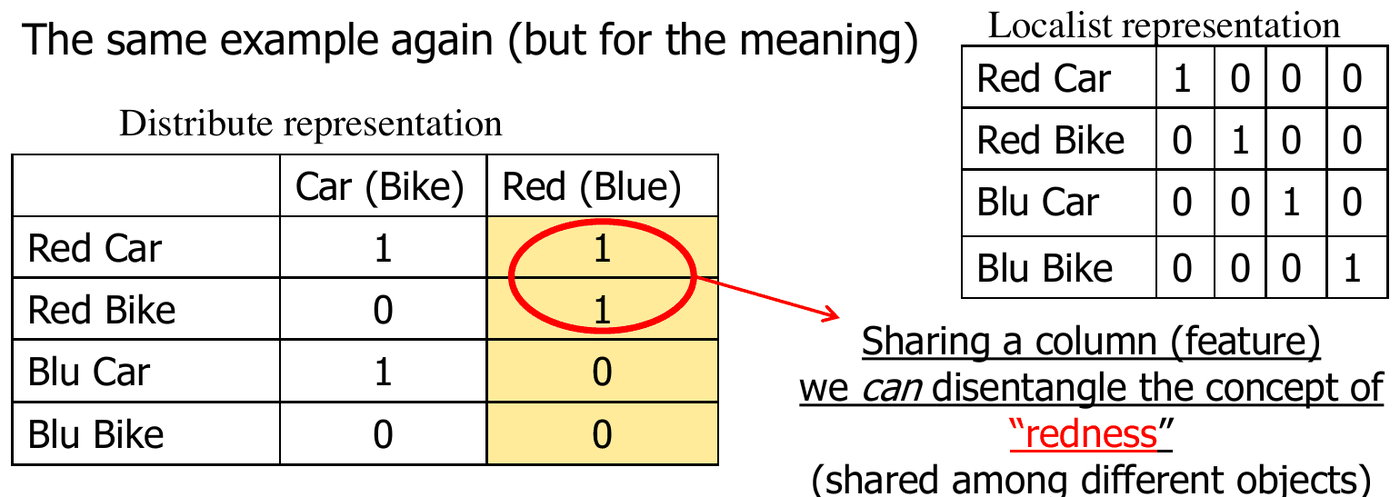
\includegraphics[width=0.80\linewidth,height=0.42\textheight,keepaspectratio]{images/17-deep_disentangling.png}
\caption{By sharing a column (feature) the concepts are disentangled.}
\end{figure}

By separating the concepts of colour and type, one can learn the
car/bike distinction or the colour \textbf{without having to see
examples of all combinations}. This \textbf{statistical separability}
makes it easy to generalise to configurations never seen: having seen
the other three cases, the blue bike is easily classified (for example
``I don't like it'' because it is not red, if the model has learned
that I like red objects); with the localist representation the blue
bike would be completely new.

With \textbf{words}: instead of a one-hot symbol per word (dimension
equal to the vocabulary), a distributed representation in which ``dog''
and ``cat'' share features allows the model to:

\begin{enumerate}
\def\labelenumi{\arabic{enumi}.}
\tightlist
\item
  \textbf{treat them similarly}: sentences with ``cat'' inform the
  predictions for sentences with ``dog'' and vice versa, transferring
  information from each training sentence to an exponential number of
  semantically related sentences (for example ``both have a tail'' →
  animal, not human);
\item
  \textbf{automatically learn that they are similar}, bringing their
  representations closer because they appear in similar contexts: this
  is \textbf{word embedding} (for example \emph{word2vec}). In the
  one-hot space every word is at distance \(\sqrt{2}\) from all the
  others; in the learned space words with similar meaning become close.
\end{enumerate}

\begin{figure}[htbp]
\centering
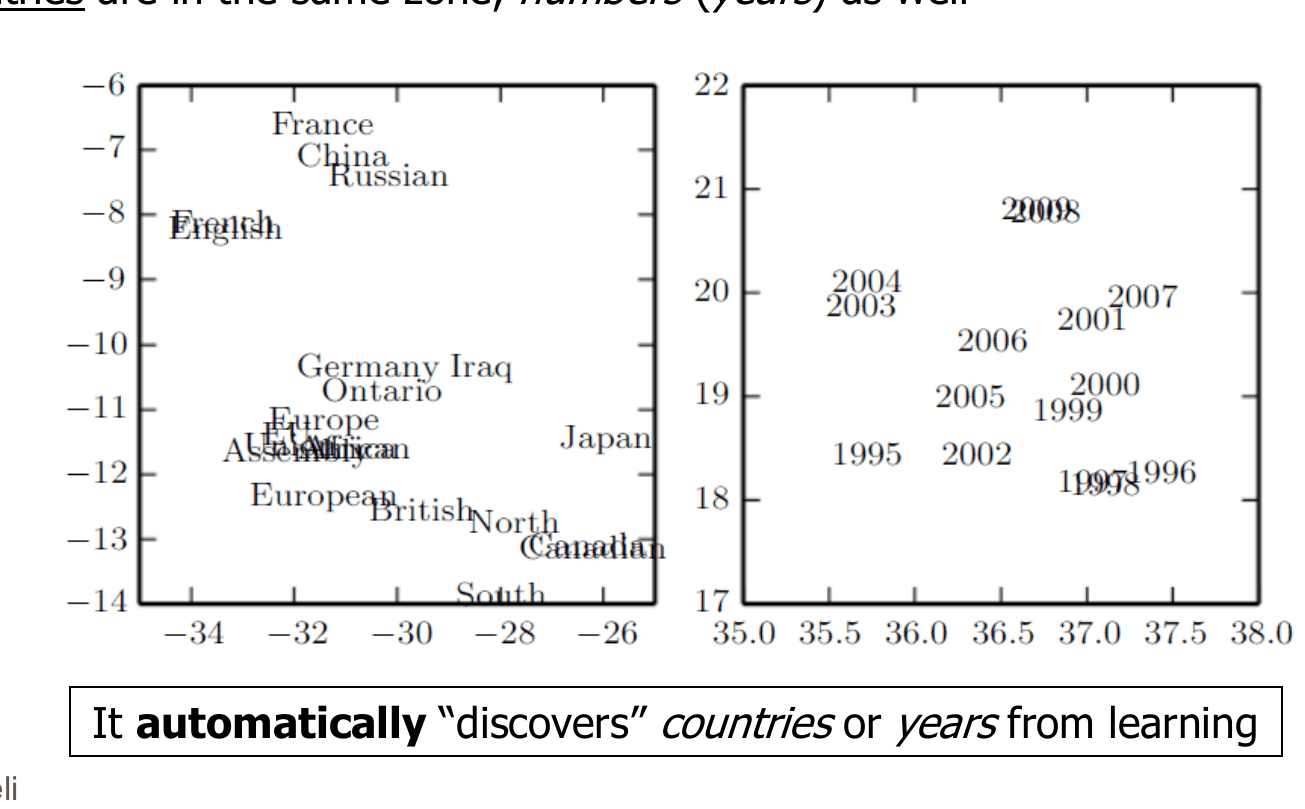
\includegraphics[width=0.69\linewidth,height=0.42\textheight,keepaspectratio]{images/17-deep_word-embedding.png}
\caption{Word embedding: semantically similar words (countries, years)
end up close together. The model automatically ``discovers'' countries
and years through learning.}
\end{figure}

\begin{boxtip}{A consideration on the results}

The model learns not only grammar (not surprising) but
\textbf{semantically meaningful} representations, and it does so
automatically, just by reading text. Why does our semantics coincide
with what the network learns? Probably language (and images)
intrinsically have a \textbf{hierarchical} structure and the deep
network has the right inductive bias to learn it in a distributed way
(real images are a tiny fraction of white-noise images). It is still an
open field.

\end{boxtip}

The debate on distributed representations extends to that between
\textbf{logical-symbolic} and \textbf{neural} paradigms for cognition:
the successes in translation cast doubt on the need for symbolic
approaches to understand sentences.

\begin{boxwarning}{Interpretability}

The other side of the coin: a distributed representation is
\textbf{less easy to interpret} than a localist one.

\end{boxwarning}

\subsection{Deep distributed
representations}\label{rappresentazioni-distribuite-profonde}

DL exploits distributed representations \textbf{across many layers},
obtained by composing levels of abstraction or a hierarchy of reused
features. Compositionality brings a further exponential gain in
statistical efficiency, in addition to that of distributed
representations: \textbf{two potentially exponential advantages} over
non-distributed and shallow models. Overall, DL models learn a
distributed representation of the data by finding (disentangling) the
\textbf{shared causal factors} that generate them, over different
levels of abstraction.

Application examples: the combination of CNNs and RNNs to generate
\textbf{image captions} (with an attention mechanism that focuses on
the part of the image related to each generated word); the
classification of \textbf{skin cancers} with a deep network trained on
130,000 cases, with competence comparable to that of dermatologists
(\emph{Nature} 2017).

\section{Further insights and recent
results}\label{altri-spunti-e-risultati-recenti}

\begin{itemize}
\tightlist
\item
  \textbf{Smoothness through structure}: with the same number of
  parameters, deeper networks impose more smoothness than shallow ones
  (each layer works on the already smooth surface produced by the
  previous one), and they seem to learn better with the same total
  number of neurons: \textbf{implicit} smoothness constraints, rather
  than explicit ones.
\item
  \textbf{The non-overfitting puzzle}: huge, over-parameterised
  networks, able to drive the training error to zero even on
  \textbf{random} labels, still generalise. One explanation: gradient
  descent imposes a form of \textbf{implicit regularisation}, with
  convergence towards the \textbf{maximum margin} solution (Poggio et
  al., 2017--2019). SGD variants with batch/weight normalisation
  maximise the normalised margin, and even standard gradient descent
  maximises the \(L^2\) margin without explicit normalisation or
  regularisation.
\item
  \textbf{Double descent}: in CNNs, ResNets and transformers, as the
  size of the model (or of the data, or the training time) grows,
  performance first improves, then worsens (the classic U) and then
  \textbf{improves again} beyond the interpolation threshold (where the
  training error becomes almost zero). The effect is often avoided with
  careful regularisation; it is not yet fully understood and is an
  important research direction. (It does not necessarily concern the
  small models of the project.)
\end{itemize}

\begin{figure}[htbp]
\centering
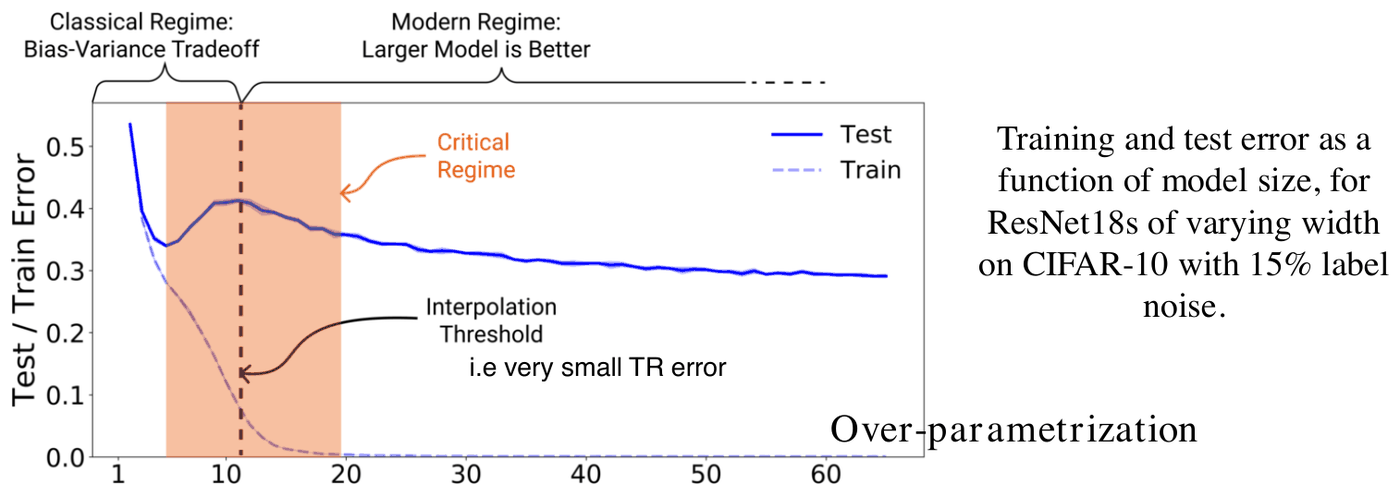
\includegraphics[width=0.80\linewidth,height=0.42\textheight,keepaspectratio]{images/17-deep_double-descent.png}
\caption{The double descent phenomenon.}
\end{figure}

\begin{figure}[htbp]
\centering
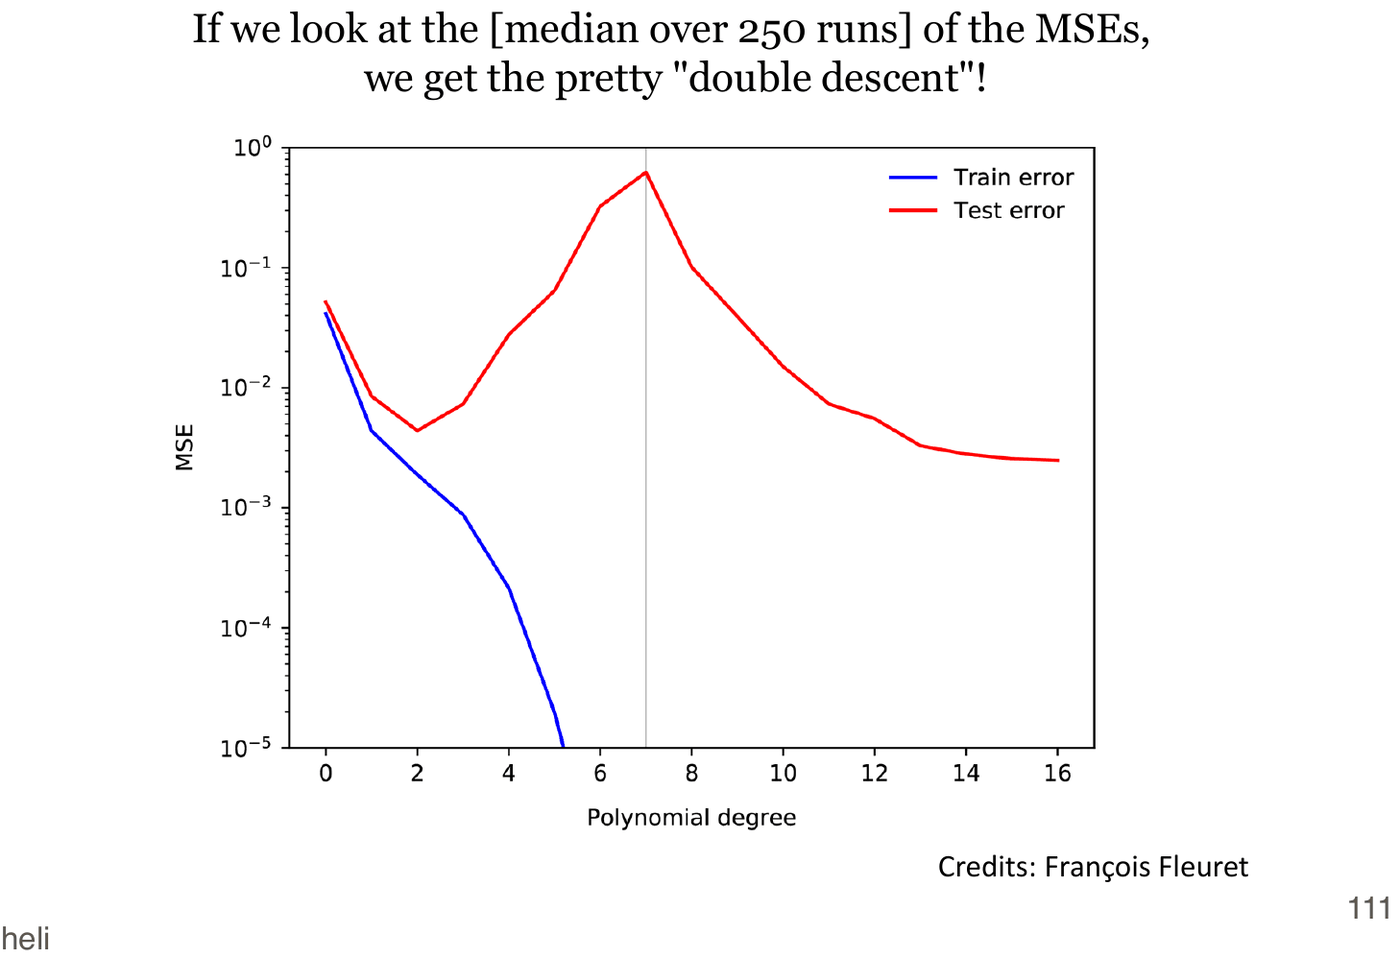
\includegraphics[width=0.54\linewidth,height=0.42\textheight,keepaspectratio]{images/17-deep_double-descent-poly.png}
\caption{A toy example with regularised polynomial regression: double
descent appears here too. Beyond zero training error, as the degree
increases the fit is driven only by the penalty term and the polynomial
becomes more and more ``piecewise linear''.}
\end{figure}

\begin{itemize}
\tightlist
\item
  \textbf{Redundancy}: in deep models there is significant redundancy
  in the parameters; given a few weights per feature the others can be
  predicted, up to more than 95\% of the weights without loss of
  accuracy (Denil et al., 2013). Parameters can also be
  \textbf{compressed} (pruning, quantisation, Huffman coding) without
  loss (Han et al., 2015): it seems that small networks are enough!
\item
  \textbf{Lottery ticket hypothesis} (Frankle and Carbin, 2018): why
  then do we train large networks? Because good performance depends on
  a \textbf{lucky initialisation} of one or more sub-networks, and
  large networks contain exponentially more of them. Retraining the
  pruned network with the same initialisation gives similar
  performance.
\item
  The role of \textbf{randomness} (randomly initialised networks and
  random-weight networks) is receiving more and more attention (see
  \href{18\%20-\%20Reti\%20neurali\%20randomizzate}{18 - Randomized
  neural networks}).
\end{itemize}

\section{Techniques}\label{tecniche}

Many layers can be hard to optimise, so the emphasis is on methods to
improve \textbf{gradient descent} (also against the \emph{vanishing
gradient}), \textbf{regularisation} (large networks) and the
\textbf{exploitation of data} (semi-supervised, reinforcement learning,
multi-task, adversarial learning\ldots). To this are added larger
datasets, public software infrastructures and hardware improvements.

\begin{boxabstract}{Key techniques for DL}

\begin{itemize}
\tightlist
\item
  Originally: \textbf{pre-training} approaches (still used in domains
  such as NLP for word embeddings).
\item
  Today (in the most popular libraries), mostly already known:

  \begin{itemize}
  \tightlist
  \item
    \textbf{SGD with momentum} (with decay of \(\eta\), mini-batch) or
    \textbf{Adam};
  \item
    \textbf{ReLU} activations in the hidden units;
  \item
    \textbf{maximum likelihood} loss (cross-entropy) with
    \textbf{softmax} at the output (also to avoid saturation and small
    gradients);
  \item
    regularisation: early stopping, weight decay, \textbf{dropout},
    \textbf{batch normalization}.
  \end{itemize}
\end{itemize}

\end{boxabstract}

\subsection{Gradient problems}\label{problemi-del-gradiente}

What happens to the norm of the gradient when it is backpropagated
through many layers?

\begin{itemize}
\tightlist
\item
  if the weights are \textbf{small}, the gradients \textbf{shrink
  exponentially} (\emph{vanishing gradient}), also because of the
  derivative of the sigmoids;
\item
  if the weights are \textbf{large}, the gradients \textbf{grow
  exponentially} (\emph{exploding gradient}).
\end{itemize}

\subsubsection{The vanishing gradient}\label{il-vanishing-gradient}

Traditional activations such as tanh have gradients in \((-1, 1)\), and
backpropagation computes the gradients with the chain rule repeated
through the layers. In a network with \(d\) layers, \(d\) of these
small numbers are multiplied to compute the gradients of the layers
close to the input: the gradient (the delta) \textbf{decreases
exponentially with \(d\)} and the layers close to the input train very
slowly.

\begin{boxnote}{Formal sketch}

If \(\mathbf{h}_l = F_l(\mathbf{h}_{l-1})\) and
\(F = F_M \circ \dots \circ F_1\), then \[
\frac{\partial F}{\partial w_l} = \frac{\partial F_M}{\partial \mathbf{h}_{M-1}}\cdots\frac{\partial F_l}{\partial w_l}, \qquad \left|\frac{\partial F}{\partial w_l}\right| \approx \rho^{M-l+1} \text{ if } \left\|\frac{\partial F_i}{\partial \mathbf{h}_i}\right\| \approx \rho.
\] With \(\rho < 1\) the gradient vanishes, with \(\rho > 1\) it
explodes.

\end{boxnote}

Approaches to tackle it range from R-prop to \emph{shortcut}
connections, to randomised networks, and ReLUs.

\subsubsection{Gradient clipping}\label{gradient-clipping}

Repeated multiplication across layers can introduce \textbf{cliffs} in
the cost function: very high derivatives that ``catapult'' the weights
very far away. \textbf{Clipping} bounds the norm of the gradient while
keeping its direction: \[
\text{if } \|\mathbf{g}\| > v \;\text{ then }\; \mathbf{g} \leftarrow \frac{v\,\mathbf{g}}{\|\mathbf{g}\|},
\] with \(v\) a threshold on the norm.

\begin{figure}[htbp]
\centering
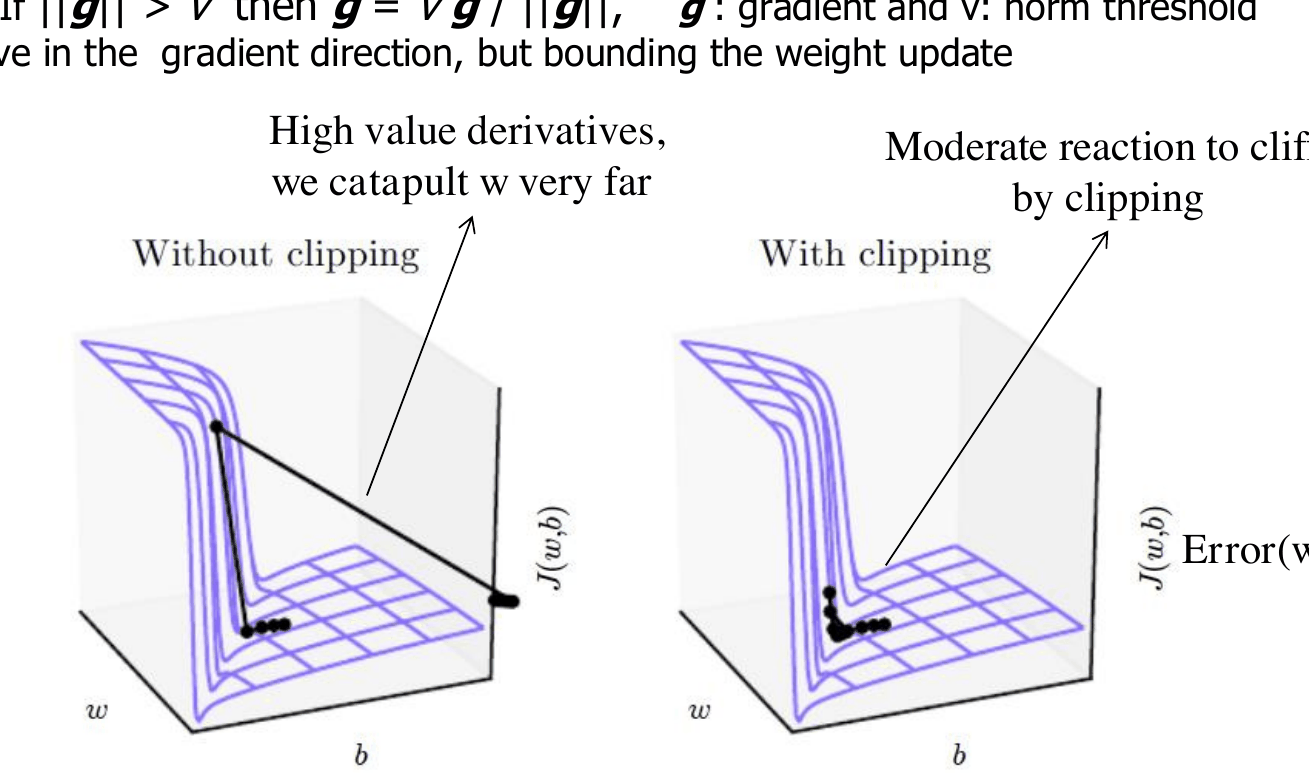
\includegraphics[width=0.69\linewidth,height=0.42\textheight,keepaspectratio]{images/17-deep_clipping.png}
\caption{Without clipping (left) and with clipping (right) when facing a
cliff of the cost function.}
\end{figure}

\subsection{ReLU}\label{relu}

\begin{boxdefinition}{ReLU (\emph{Rectified Linear Unit})}

\[
f(x) = \max(0, x) = \begin{cases} 0 & x < 0 \\ x & x \ge 0. \end{cases}
\]

\end{boxdefinition}

Why use it in DL (since 2009)?

\begin{itemize}
\tightlist
\item
  Better \textbf{gradient propagation} through many layers: it avoids
  the saturation of sigmoids, because \(f'(x) = 1\) for every positive
  net.
\item
  \textbf{Sparse activation}: in a randomly initialised network about
  50\% of the hidden units are active (non-zero output).
\item
  \textbf{Efficient computation}: only comparisons, sums and products.
\item
  It still has a neuroscientific inspiration, and it allows faster and
  more effective training of deep networks.
\end{itemize}

ReLU is \textbf{not differentiable at 0}, but in libraries the
derivative is usually assumed to be 0 (left) or 1 (right): the
approximation is acceptable and safe, because with numerical
approximations it is unlikely to evaluate exactly \(f(0)\). (A more
rigorous approach uses non-differentiable optimisation for piecewise
linear functions.)

A trick: start with \textbf{positive nets}, for example with small
positive biases (0.1), so that ReLUs are initially active for most
inputs and let the derivatives through.

Variants: \textbf{ELU} (\emph{Exponential Linear Unit}),
\(f(x) = \alpha(e^x - 1)\) for \(x \le 0\) and \(x\) for \(x > 0\);
\textbf{Leaky ReLU}, \(f(x) = 0.01x\) for \(x < 0\) and \(x\) for
\(x \ge 0\). They also learn on the left side (neurons do not ``die'')
and have mean activation closer to zero. Many variants have comparable
performance; in general they avoid some defects while keeping the
linear part, which makes the model easier to optimise.

\subsection{Batch normalization}\label{batch-normalization}

\textbf{Batch normalization} normalises each mini-batch by computing
its statistics (mean and variance) for each layer: the matrix
{[}examples of the batch × activations of the units{]} is normalised to
zero mean and unit variance, and the transformation is included in
backpropagation. Just as normalising the input is standard practice,
BN keeps the data flowing between the intermediate layers normalised.
Effects: \textbf{regularisation} (due to the noise introduced by the
mini-batch) and \textbf{faster learning} with higher accuracy (relevant
because it made it possible to effectively train CNNs and deep models
with sigmoids). (Details not required for the exam, unless it is
used.)

\subsection{Dropout}\label{dropout}

\textbf{Dropout} randomly selects a subset of the network during
training. It is explained by two concepts already known:
\textbf{ensembles} (an implicit bagging of different sub-networks, but
computationally cheap) and \textbf{regularisation}.

Bagging trains \(n\) models on different subsets of the training set
and averages their outputs: high-variance, low-bias models work well on
average. Dropout approximates and exploits this process with an
\textbf{exponential} number of sub-networks, while having \textbf{a
single network} at test time, and it maximises the diversity of the
ensemble by avoiding complex co-adaptations on the training data.

\begin{figure}[htbp]
\centering
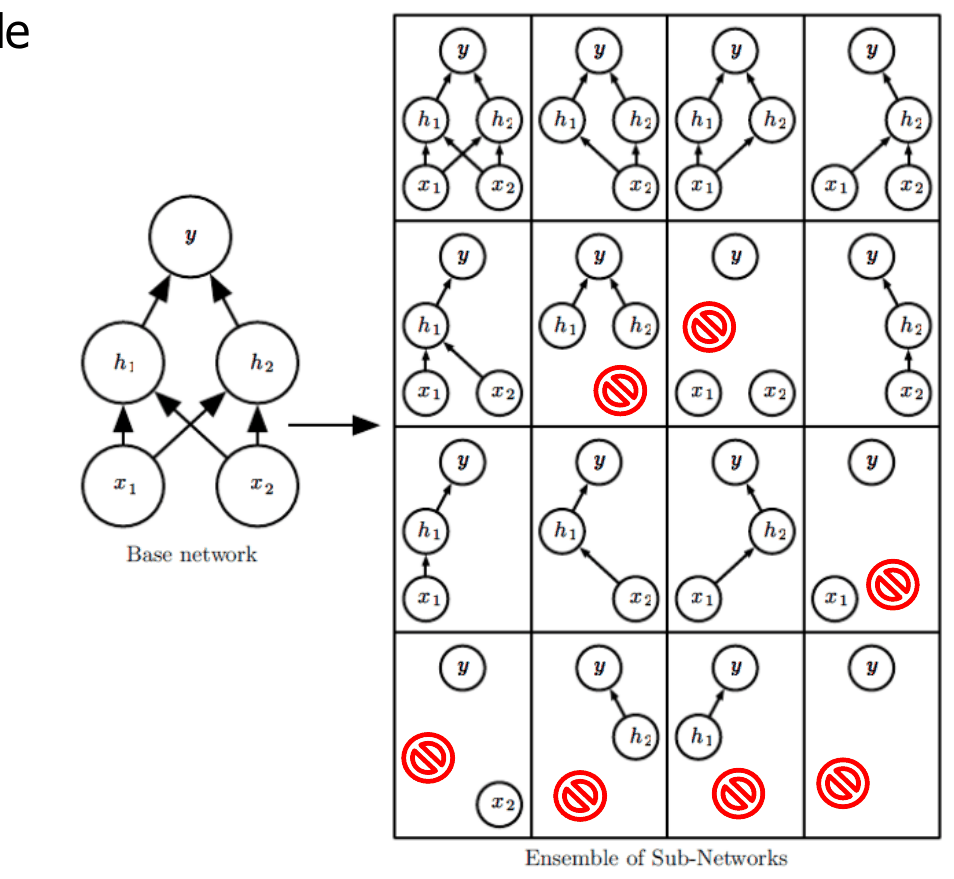
\includegraphics[width=0.51\linewidth,height=0.42\textheight,keepaspectratio]{images/17-deep_dropout.png}
\caption{Dropout trains the ensemble of all the sub-networks obtainable
by removing non-output units from the base network. Some sub-networks
do not work, but in large networks it is unlikely that there is no path
from input to output.}
\end{figure}

\begin{boxabstract}{Dropout algorithm}

\begin{itemize}
\tightlist
\item
  Each time an example is loaded into a mini-batch, a different
  \textbf{binary mask} is sampled to be applied to all input and hidden
  units, independently for each unit. The probability of including a
  unit is a hyperparameter (typically 0.8 for the input and 0.5 for the
  hidden units).
\item
  Each unit is multiplied by its mask (zero is equivalent to removing
  it, \emph{drop out}): a sub-network is obtained.
\item
  Forward pass, backpropagation and update are performed as usual,
  training a subset of units at a time.
\item
  The removed units are then reinserted with their original weights.
\end{itemize}

\end{boxabstract}

Only a small fraction of the sub-networks is trained (each for a single
step), but \textbf{parameter sharing} means that the others also reach
good parameters: an exponential number of models is handled with
tractable memory. To approximate the prediction of the ensemble at test
time the \emph{weight scaling inference rule} is used: the weights are
multiplied by the inclusion probability (typically 0.5), so that the
expected output of each unit is the same as in training.

Regularising effect: it avoids training all units on all data by
reducing their interactions (and diversifying them, as committees
require); it reduces variance like bagging; it injects
\textbf{structured noise} (for example recognising a face without the
unit that detects the nose). Above all, it regularises each unit to be
not only a good feature, but \textbf{a feature that is good in many
contexts} (different sub-networks). For linear regression it is
equivalent to \(L^2\) weight decay with a different \(\lambda\) for
each input. It can be used with any distributed-representation model
trained with SGD.

\subsection{L1 regularisation}\label{regolarizzazione-l1}

Using the \(L^1\) norm (sum of absolute values) instead of \(L^2\) in
the penalty (for linear models it is \textbf{LASSO}) favours the
\textbf{elimination} of features (weights exactly at zero), whereas
\(L^2\) usually only reduces the magnitude of the weights: simpler
models are obtained. The solution requires non-differentiable
optimisation techniques (sub-gradient, smooth approximations of the
\(L^1\) norm\ldots).

\begin{figure}[htbp]
\centering
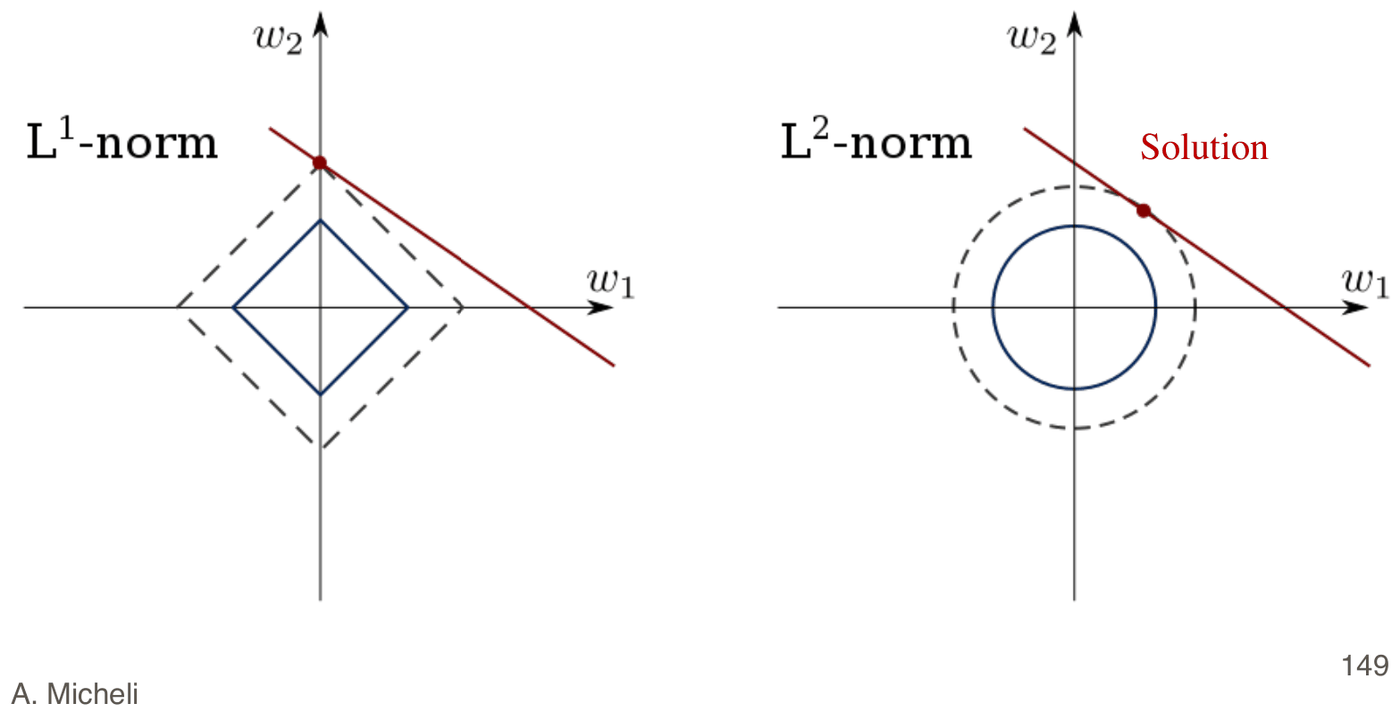
\includegraphics[width=0.74\linewidth,height=0.42\textheight,keepaspectratio]{images/17-deep_l1-l2.png}
\caption{Why L1 produces sparse solutions: the level curves of the L1
norm have ``corners'' on the axes, where one coordinate is zero.}
\end{figure}

\subsection{Adversarial learning}\label{apprendimento-avversario}

\textbf{Generative Adversarial Networks} (GANs) are two networks in
competition: one \textbf{generates} candidates, the other
\textbf{evaluates} them (distinguishing real from generated ones). They
are used for example to generate photorealistic images of people who do
not exist.

\section{Applications, challenges and
conclusions}\label{applicazioni-sfide-e-conclusioni}

DL is successful in \textbf{NLP} (speech recognition, translation,
sentiment analysis, question answering\ldots), in \textbf{computer
vision} (images and video: object recognition, medical applications,
image synthesis\ldots) with performance never reached before, and in
the game of \textbf{Go}. It is discussed in more depth in the NLP and
ISPR courses.

Open challenges: theoretical analysis and framework; optimal
architecture design (how many layers? which units? cross-validation may
be too expensive); efficiency for big data; stream (on-line)
processing; structured data (sequences, trees, graphs).

Hardware has changed too: Google TPUs (initially only for inference),
Nvidia GPUs, NPUs in smartphone chips (Huawei Kirin 970), Apple's
\emph{Neural Engine} (since 2017).

\begin{boxabstract}{Summary}

\begin{itemize}
\tightlist
\item
  Technical progress and the availability of data have made it possible
  to learn with deep and very large networks, with state-of-the-art
  results especially where the \textbf{compositionality} of features is
  relevant (vision, language).
\item
  Two potentially exponential advantages: \textbf{depth} (composition
  of functions, no-flattening) and \textbf{distributed representations}
  (shared attributes).
\item
  The most general concept to emerge is \textbf{representation
  learning}.
\item
  Techniques: ReLU, cross-entropy with softmax, SGD with momentum/Adam,
  dropout, batch normalization, gradient clipping.
\item
  ML makes it relatively easier to develop sophisticated AI systems
  (and software in general) for real problems.
\end{itemize}

\end{boxabstract}

\begin{boxquestion}{Possible exam questions}

\begin{itemize}
\tightlist
\item
  What is meant by deep learning? What are the aspects common to the
  various approaches?
\item
  Are many layers really needed? Discuss the parity example and the
  no-flattening results.
\item
  What is the inductive bias of deep models?
\item
  What is representation learning? Pre-training and transfer learning.
\item
  What is an autoencoder?
\item
  Symbolic versus distributed representations: advantages of the
  latter.
\item
  What is the vanishing gradient? How is it tackled (ReLU,
  clipping\ldots)?
\item
  Describe dropout and explain its regularising effect.
\end{itemize}

\end{boxquestion}
